\chapter{Evaluation}

In order to evaluate the proposed control method, we create the simulation platform using MATLAB and VREP (Coppelia Sim). The problem configuration is a group of five unicycle-type agents cover a convex bounded region with a constant heading velocity. They are not allowed to get out of the region during the operation and the rotation velocity is limited. Figure \ref{fig:VREP} depicts the scenario of this coverage problem. 
\begin{figure} [h]
	\centering
	\includegraphics[width=1\linewidth]{VREP_SIM}
	\caption{5 Agents - Convex region}
	\label{fig:VREP}
\end{figure}

During the operation, all data of agents are logged for the evaluation. Data such as virtual mass's position and control input, are plotted intuitively. Figure \ref{fig:VREP_state} demonstrates the trajectories of five agents created throughout the operation. They never cross the boundary lines, this implies the state constraint is not violated. \\
\begin{figure} [!h]
	\centering
	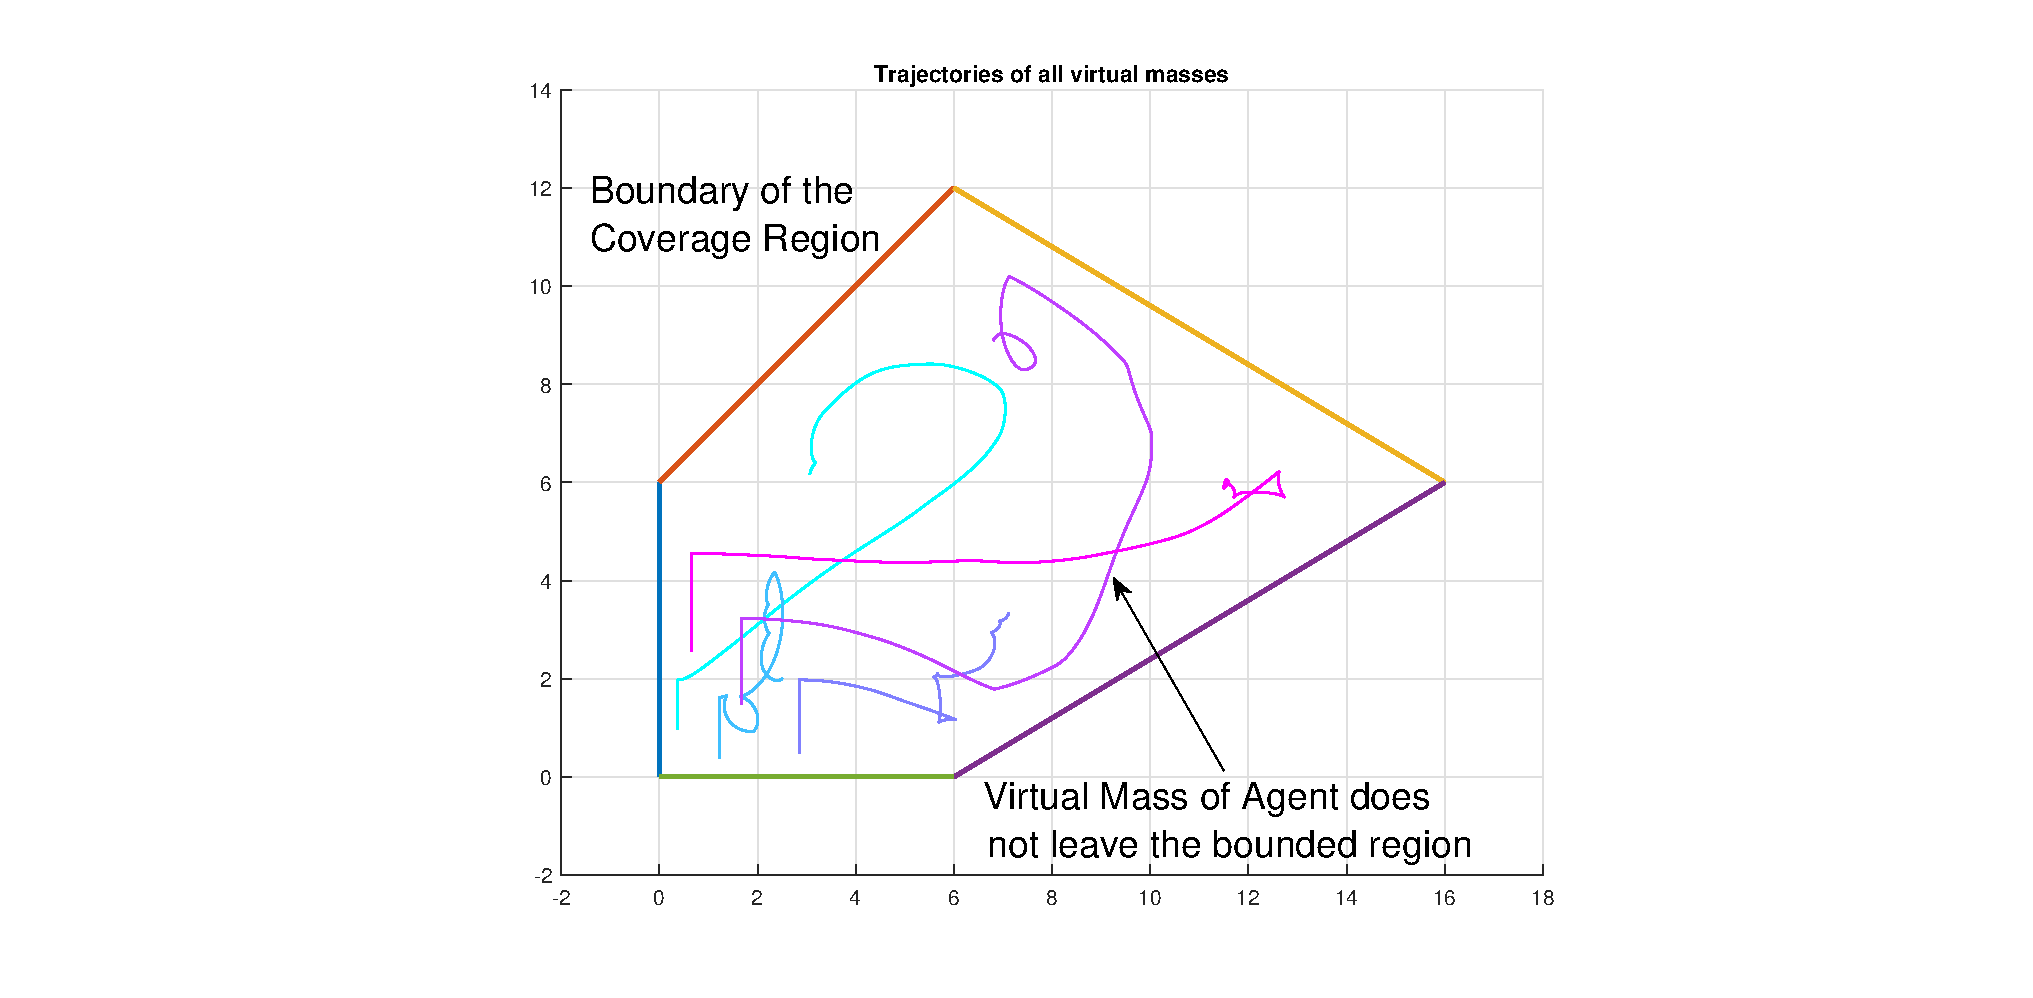
\includegraphics[width=1.3\linewidth]{Eva_VREP_trajectories}
	\caption{Feasibility of States}
	\label{fig:VREP_state}
\end{figure}

\begin{figure} [!h]
	\centering
	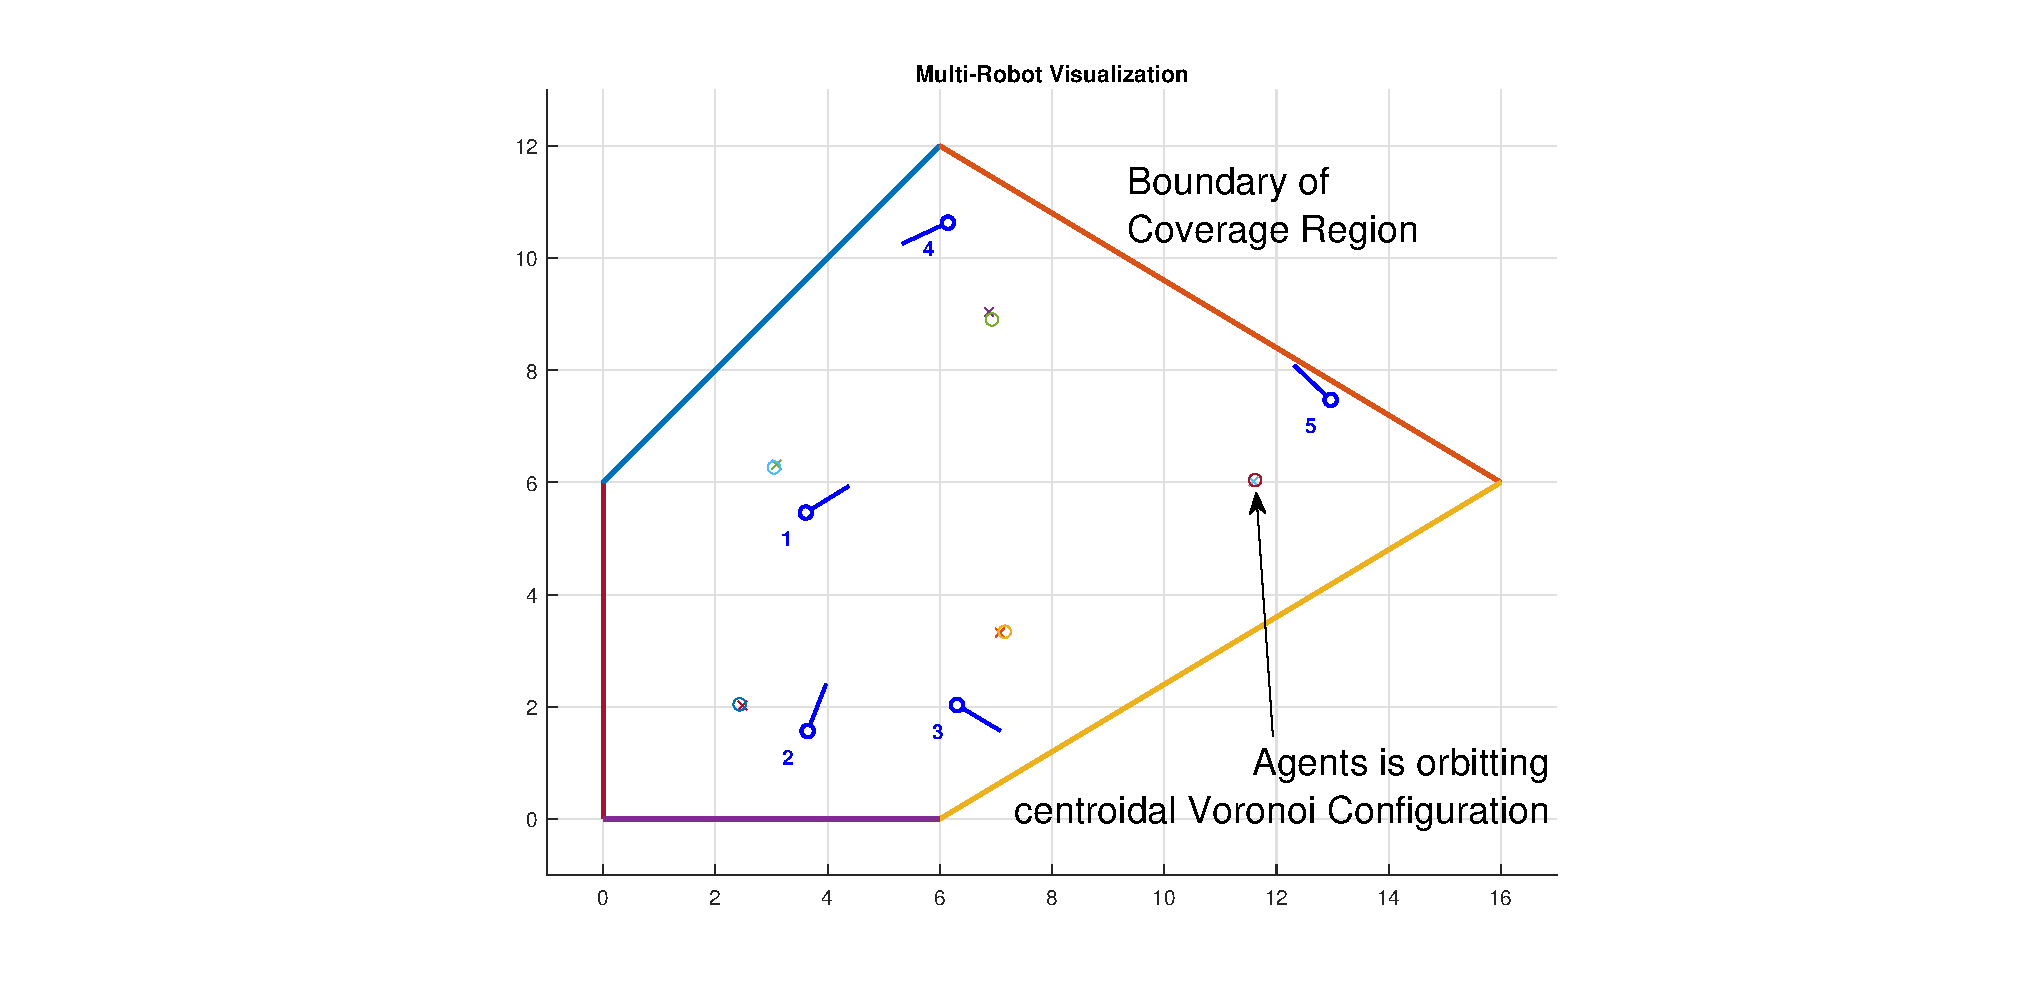
\includegraphics[width=1.3\linewidth]{Eva_VREP_bot_final}
	\caption{Final State of the Coverage Control}
	\label{fig:VREP_bot_final}
\end{figure}
Figure \ref{fig:VREP_bot_final} and \ref{fig:VREP_voronoi} depicts the final state of the coverage problem. It can be seen that all agents are orbiting their virtual masses, which converge to the set of centroidal Voronoi configuration. \\
\begin{figure} [!h]
	\centering
	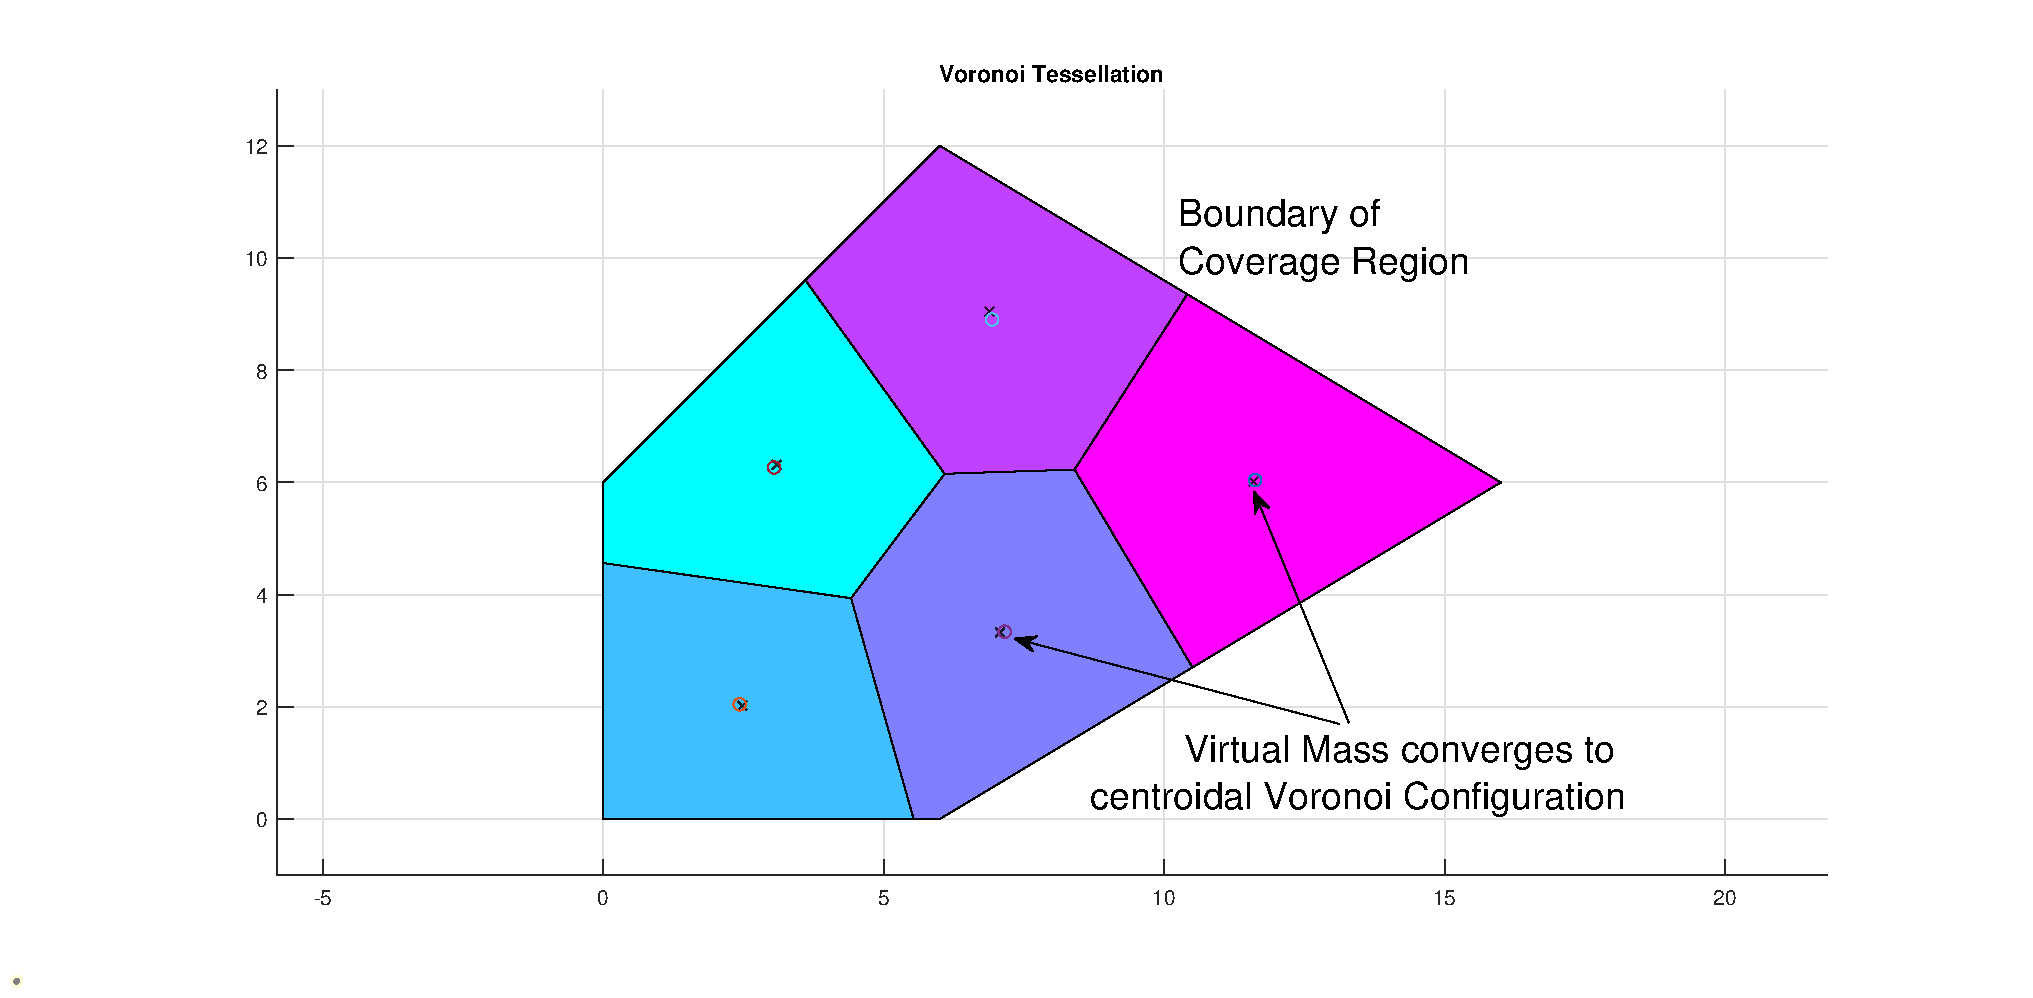
\includegraphics[width=1\linewidth]{Eva_VREP_Voronoi}
	\caption{Agents Orbit the Centroidal Voronoi Configuration}
	\label{fig:VREP_voronoi}
\end{figure}

The maximal rotation velocity of agents are configured to be -0.5 rad/s and 0.5 rad/s. As can be seen in Figure \ref{fig:VREP_control_input} that the control input is always inside the red bounded lines, this indicates that the input constraint are never violated. \\
\begin{figure} [!h]
	\centering
	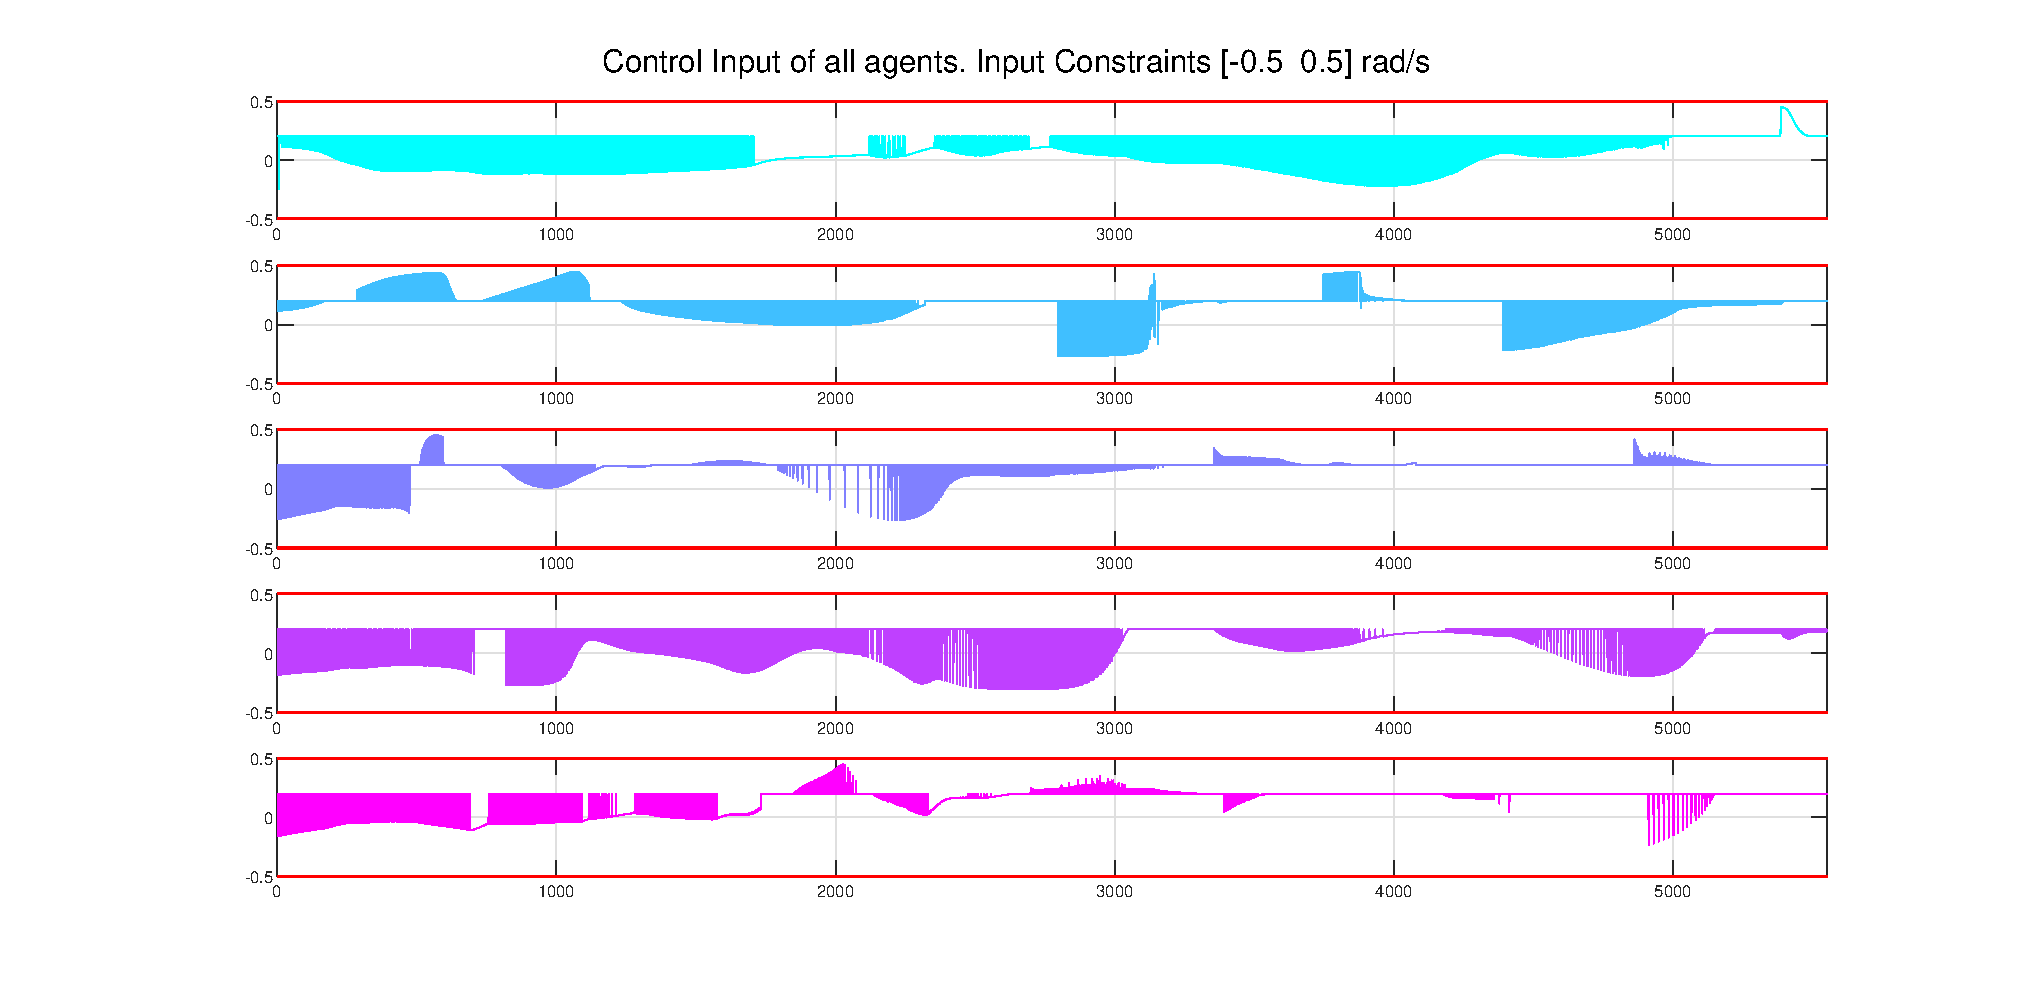
\includegraphics[width=1\linewidth]{Eva_VREP_control_input}
	\caption{Feasible Control Input}
	\label{fig:VREP_control_input}
\end{figure}

Using this simulation environment, we also evaluate the coverage problem with different convex regions such as triangle or rectangle form. The results depicts the reliability and feasibility of the proposed control method.